\documentclass[11pt]{article}
\usepackage{tikz}
\usepackage{geometry}
\usepackage{amssymb}
\geometry{letterpaper, landscape, margin=0.5in}
\usetikzlibrary{positioning, calc}

\begin{document}

\begin{center}
{\Huge \textbf{THE PROFANE TEMPLE OF DEMETER}}\\[0.3em]
{\Large Level 4: The Sealed Depths}
\end{center}

\vspace{0.5em}

\begin{center}
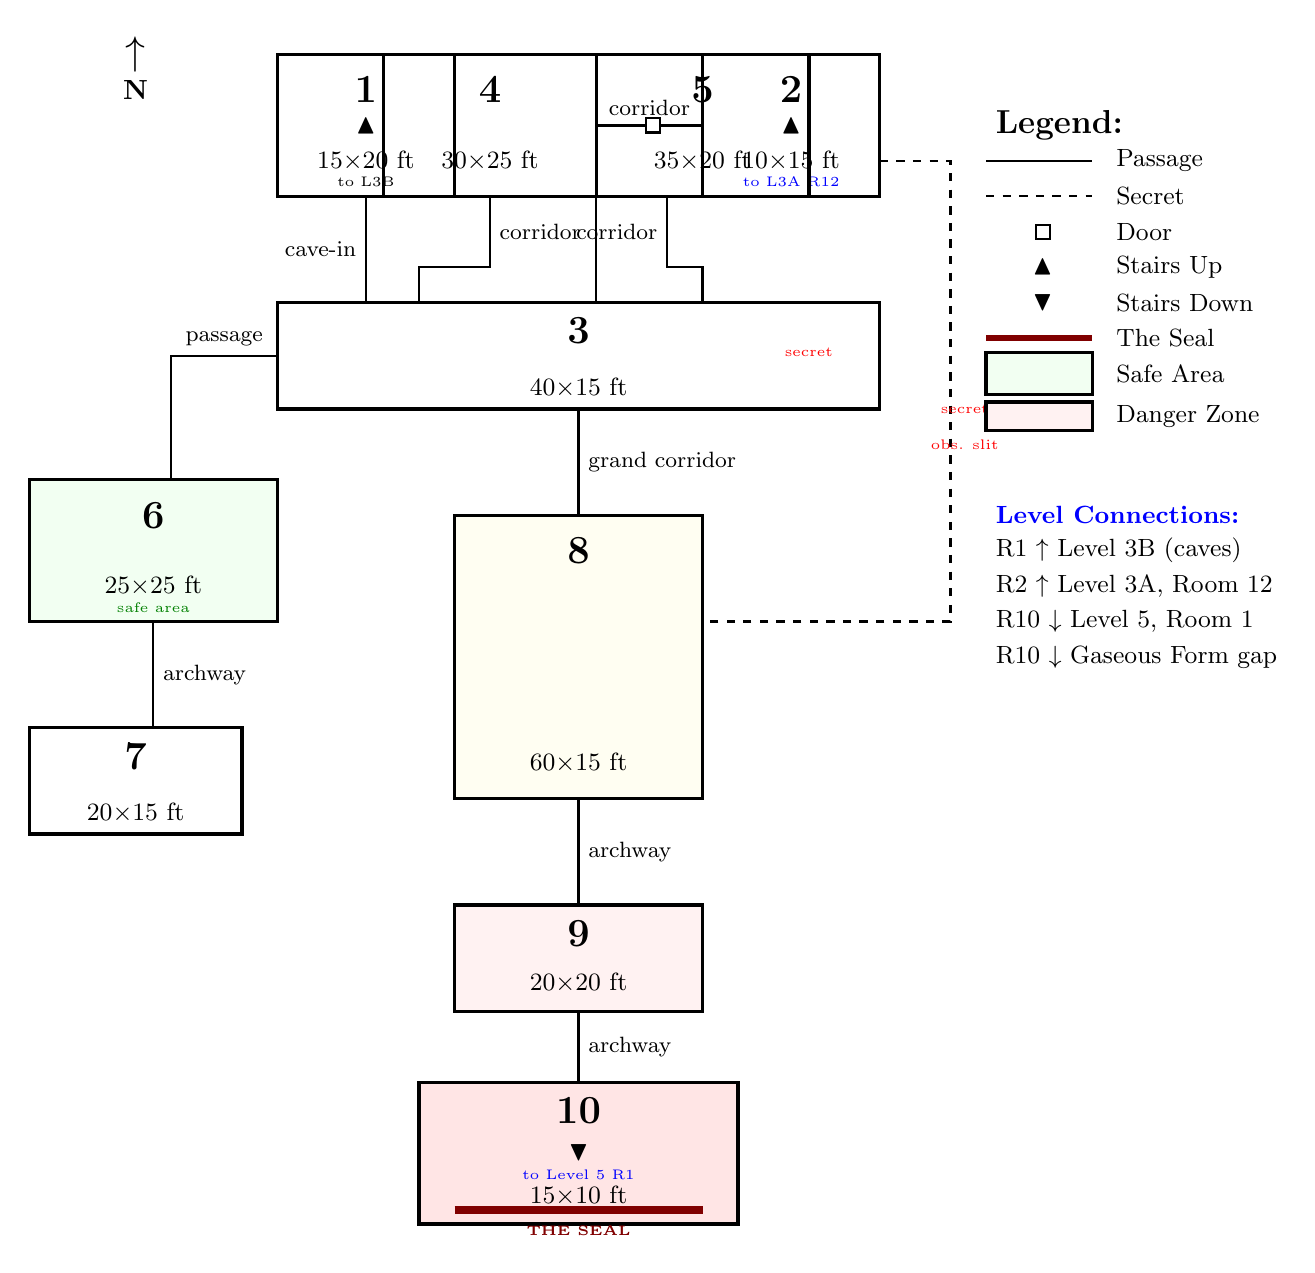
\begin{tikzpicture}[scale=0.9]

% North arrow
\node at (-2,11) {\Large $\uparrow$};
\node at (-2,10.5) {\textbf{N}};

% ============================================================
% ARRIVAL ZONE (top section)
% ============================================================

% ROOM 1: The Frozen Stair (top-left)
\draw[very thick] (0,9) rectangle (2.5,11);
\node at (1.25,10.5) {\Large \textbf{1}};
\node[font=\small] at (1.25,9.5) {15$\times$20 ft};
\node at (1.25,10) {$\blacktriangle$};
\node[font=\tiny] at (1.25,9.2) {to L3B};

% ROOM 2: The Priest's Landing (top-right)
\draw[very thick] (6,9) rectangle (8.5,11);
\node at (7.25,10.5) {\Large \textbf{2}};
\node[font=\small] at (7.25,9.5) {10$\times$15 ft};
\node at (7.25,10) {$\blacktriangle$};
\node[font=\tiny, blue] at (7.25,9.2) {to L3A R12};

% Connection Room 1 to Room 3 (south)
\draw[thick] (1.25,9) -- (1.25,7.5);
\node[left,font=\footnotesize] at (1.25,8.25) {cave-in};

% Connection Room 2 to Room 3 (locked bronze door, west)
\draw[thick] (6,10) -- (4.5,10) -- (4.5,7.5);
\node[above,font=\footnotesize] at (5.25,10) {corridor};
\fill[white,draw=black,thick] (5.2,9.9) rectangle (5.4,10.1);

% ============================================================
% ROOM 3: The Junction Hall (central horizontal corridor)
% ============================================================
\draw[very thick] (0,6) rectangle (8.5,7.5);
\node at (4.25,7.1) {\Large \textbf{3}};
\node[font=\small] at (4.25,6.3) {40$\times$15 ft};

% Secret alcove in Room 3
\node[font=\tiny,red] at (7.5,6.8) {secret};

% ============================================================
% THE PRIESTS' QUARTERS (north branches off Junction Hall)
% ============================================================

% Connection Room 3 to Room 4 (north, from left side of junction)
\draw[thick] (2,7.5) -- (2,8) -- (3,8) -- (3,9);
\node[right,font=\footnotesize] at (3,8.5) {corridor};

% ROOM 4: The Dormitory of the Faithful
\draw[very thick] (1.5,9) rectangle (4.5,11);
\node at (3,10.5) {\Large \textbf{4}};
\node[font=\small] at (3,9.5) {30$\times$25 ft};

% Connection Room 3 to Room 5 (north, from right side of junction)
\draw[thick] (6,7.5) -- (6,8) -- (5.5,8) -- (5.5,9);
\node[left,font=\footnotesize] at (5.5,8.5) {corridor};

% ROOM 5: The Refectory
\draw[very thick] (4.5,9) rectangle (7.5,11);
\node at (6,10.5) {\Large \textbf{5}};
\node[font=\small] at (6,9.5) {35$\times$20 ft};

% ============================================================
% THE SHRINE (west branches off Junction Hall)
% ============================================================

% Connection Room 3 to Room 6 (west)
\draw[thick] (0,6.75) -- (-1.5,6.75) -- (-1.5,5);
\node[above,font=\footnotesize] at (-0.75,6.75) {passage};

% ROOM 6: The Shrine of Archon Kleistos
\draw[very thick, fill=green!5] (-3.5,3) rectangle (0,5);
\node at (-1.75,4.5) {\Large \textbf{6}};
\node[font=\small] at (-1.75,3.5) {25$\times$25 ft};
\node[font=\tiny,green!50!black] at (-1.75,3.2) {safe area};

% Connection Room 6 to Room 7 (south, through curtain)
\draw[thick] (-1.75,3) -- (-1.75,1.5);
\node[right,font=\footnotesize] at (-1.75,2.25) {archway};

% ROOM 7: The Ritual Vestry
\draw[very thick] (-3.5,0) rectangle (-0.5,1.5);
\node at (-2,1.1) {\Large \textbf{7}};
\node[font=\small] at (-2,0.3) {20$\times$15 ft};

% ============================================================
% THE APPROACH (south from Junction Hall)
% ============================================================

% Connection Room 3 to Room 8 (south, main corridor)
\draw[thick] (4.25,6) -- (4.25,4.5);
\node[right,font=\footnotesize] at (4.25,5.25) {grand corridor};

% ROOM 8: The Hall of Wards (long vertical corridor)
\draw[very thick, fill=yellow!5] (2.5,0.5) rectangle (6,4.5);
\node at (4.25,4) {\Large \textbf{8}};
\node[font=\small] at (4.25,1) {60$\times$15 ft};

% Secret observation slit from Room 2 to Room 8
\draw[thick,dashed] (8.5,9.5) -- (9.5,9.5) -- (9.5,3) -- (6,3);
\node[font=\tiny,red] at (9.7,6) {secret};
\node[font=\tiny,red] at (9.7,5.5) {obs. slit};

% Connection Room 8 to Room 9 (south)
\draw[thick] (4.25,0.5) -- (4.25,-1);
\node[right,font=\footnotesize] at (4.25,-0.25) {archway};

% ROOM 9: The Antechamber of Despair
\draw[very thick, fill=red!5] (2.5,-2.5) rectangle (6,-1);
\node at (4.25,-1.4) {\Large \textbf{9}};
\node[font=\small] at (4.25,-2.1) {20$\times$20 ft};

% Connection Room 9 to Room 10 (south)
\draw[thick] (4.25,-2.5) -- (4.25,-3.5);
\node[right,font=\footnotesize] at (4.25,-3) {archway};

% ROOM 10: The Sealed Doors
\draw[very thick, fill=red!10] (2,-5.5) rectangle (6.5,-3.5);
\node at (4.25,-3.9) {\Large \textbf{10}};
\node[font=\small] at (4.25,-5.1) {15$\times$10 ft};
\node at (4.25,-4.5) {$\blacktriangledown$};
\node[font=\tiny, blue] at (4.25,-4.8) {to Level 5 R1};

% The Sealed Doors visual indicator
\draw[line width=3pt, red!50!black] (2.5,-5.3) -- (6,-5.3);
\node[font=\tiny, red!50!black] at (4.25,-5.6) {\textbf{THE SEAL}};

% ============================================================
% LEGEND
% ============================================================

\node[anchor=west,font=\large] at (10,10) {\textbf{Legend:}};

\draw[thick] (10,9.5) -- (11.5,9.5);
\node[anchor=west,font=\small] at (11.7,9.5) {Passage};

\draw[thick,dashed] (10,9) -- (11.5,9);
\node[anchor=west,font=\small] at (11.7,9) {Secret};

\fill[white,draw=black,thick] (10.7,8.4) rectangle (10.9,8.6);
\node[anchor=west,font=\small] at (11.7,8.5) {Door};

\node at (10.8,8) {$\blacktriangle$};
\node[anchor=west,font=\small] at (11.7,8) {Stairs Up};

\node at (10.8,7.5) {$\blacktriangledown$};
\node[anchor=west,font=\small] at (11.7,7.5) {Stairs Down};

\draw[line width=2pt, red!50!black] (10,7) -- (11.5,7);
\node[anchor=west,font=\small] at (11.7,7) {The Seal};

\draw[very thick, fill=green!5] (10,6.2) rectangle (11.5,6.8);
\node[anchor=west,font=\small] at (11.7,6.5) {Safe Area};

\draw[very thick, fill=red!5] (10,5.7) rectangle (11.5,6.1);
\node[anchor=west,font=\small] at (11.7,5.9) {Danger Zone};

% ============================================================
% LEVEL CONNECTION ANNOTATIONS
% ============================================================

\node[font=\small, blue, anchor=west] at (10,4.5) {\textbf{Level Connections:}};
\node[font=\small, anchor=west] at (10,4) {R1 $\uparrow$ Level 3B (caves)};
\node[font=\small, anchor=west] at (10,3.5) {R2 $\uparrow$ Level 3A, Room 12};
\node[font=\small, anchor=west] at (10,3) {R10 $\downarrow$ Level 5, Room 1};
\node[font=\small, anchor=west] at (10,2.5) {R10 $\downarrow$ Gaseous Form gap};

\end{tikzpicture}
\end{center}

\vspace{0.5em}

\section*{Room Key}
\begin{enumerate}
    \item \textbf{The Frozen Stair} (15$\times$20 ft) --- Natural cave descent from Level 3B, icy chimney
    \item \textbf{The Priest's Landing} (10$\times$15 ft) --- Warded arrival from Level 3A R12, observation slit
    \item \textbf{The Junction Hall} (40$\times$15 ft) --- Central vaulted corridor, processional frieze, hidden cache
    \item \textbf{The Dormitory of the Faithful} (30$\times$25 ft) --- Ruined quarters, Wraith of Brother Lysandros
    \item \textbf{The Refectory} (35$\times$20 ft) --- Cursed feast hall, 4 Ghouls, \textit{Potion of Extra-Healing}
    \item \textbf{The Shrine of Archon Kleistos} (25$\times$25 ft) --- Spirit of Kleistos, \textit{Ring of Spell Storing}, safe area
    \item \textbf{The Ritual Vestry} (20$\times$15 ft) --- Consecrated oil, Shadow guardian, key to Room 2
    \item \textbf{The Hall of Wards} (60$\times$15 ft) --- Failing ward-glyphs, 2 Spectres, master-ward blessing
    \item \textbf{The Antechamber of Despair} (20$\times$20 ft) --- Corruption test, Adrianna's visions
    \item \textbf{The Sealed Doors} (15$\times$10 ft) --- The seal itself, descent to Level 5
\end{enumerate}

\end{document}
